% Configure documentclass
\documentclass[a4paper,12pt,twoside]{report}

% Add common preamble to the document
%% This file is shared between thesis and proposal

\usepackage[scaled]{helvet}
\usepackage{url}
\usepackage{cite}
\usepackage{listings}
\usepackage[pdftex]{graphicx}
\usepackage[hang,small,bf]{caption}
\usepackage{styles/tum}
\usepackage{setspace}
\usepackage[german,english]{babel}
\usepackage{float}
\usepackage{floatflt}
\usepackage{fancyhdr}
\usepackage{color}
\usepackage{booktabs}
\usepackage[pdftex,bookmarks=true,plainpages=false,pdfpagelabels=true]{hyperref}	%TODO make yourself familiar with \label, \ref and \hyperref for referencing figures, tables, chapters, etc.
\usepackage{mdwlist}
\usepackage{enumerate}
\usepackage{array}
\usepackage{longtable}
\usepackage[utf8]{inputenc}
\usepackage[capitalize, noabbrev]{cleveref}
\usepackage{wasysym}
\usepackage{todonotes}

% Path for graphics
\graphicspath{{figures/}}

% Include the Thesis metadata like title, author, etc. 
\input{metadata}

%%%%%%%%%%%%%%%%%%%%%%%%%%%%%%%%%%%%%%%%%%%%%%%%%%%%%%%%%%%%%%%%%%%%%%%%%%%%%%%%%%%%%%%%%%%%%%%%%
% Custom Commands for this template
%%%%%%%%%%%%%%%%%%%%%%%%%%%%%%%%%%%%%%%%%%%%%%%%%%%%%%%%%%%%%%%%%%%%%%%%%%%%%%%%%%%%%%%%%%%%%%%%%

% Annotate feedback you received 
\newcommand{\feedback}[1]{\todo[inline,color=green,caption={}]{#1}}

% State what is missing in this spot
\newcommand{\missing}[1]{\todo[inline,color=yellow,caption={}]{#1}}

% Inline to do note: 
\newcommand{\TODO}[1]{\todo[inline,caption={}]{#1}}






%%%%%%%%%%%%%%%%%%%%%%%%%%%%%%%%%%%%%%%%%%%%%%%%%%%%%%%%%%%
% Theses specific packages go here
%%%%%%%%%%%%%%%%%%%%%%%%%%%%%%%%%%%%%%%%%%%%%%%%%%%%%%%%%%%
\usepackage[printonlyused]{acronym}


%%%%%%%%%%%%%%%%%%%%%%%%%%%%%%%%%%%%%%%%%%%%%%%%%%%%%%%%%%%
% Begin of document
%%%%%%%%%%%%%%%%%%%%%%%%%%%%%%%%%%%%%%%%%%%%%%%%%%%%%%%%%%%

\begin{document}
\setlength{\evensidemargin}{22pt}
\setlength{\oddsidemargin}{22pt}


\hypersetup{pdfborder={0 0 0}, pdfauthor={\author}, pdftitle={\title}}

\lstset{showspaces=false, numbers=left, frame=single, basicstyle=\small}

\pagenumbering{alph}

%------- Cover and Title setup -------
\thispagestyle{empty}
{
\sffamily

\vspace{4cm}
\begin{center}
\oTUM{4cm}

\vspace{5mm}     
{\LARGE \bf \sffamily Technical University of Munich}

\vspace{5mm}
{\Large School of Computation, Information and Technology \\ -- Informatics -- }
\vspace{1mm}
\end{center}

\vspace{15mm}

\begin{center}
{\large {\degree}'s Thesis in \program}
\vspace{2cm}

\begin{spacing}{1.5}
{\huge\bf \sffamily  \title}\\%[3ex]
\end{spacing}

\vspace{15mm}
{\LARGE \author}

\end{center}
}

\thispagestyle{empty}
{
\sffamily

\vspace{1cm}
\begin{center}
\oTUM{4cm}

\vspace{5mm}     
{\LARGE \bf \sffamily Technical University of Munich}

\vspace{5mm}
{\Large School of Computation, Information and Technology \\ -- Informatics -- }	
\vspace{1mm}
\end{center}

\vspace{15mm}

\begin{center}
        {\large {\proposal} {\degree}'s Thesis in \program}
\vspace{8mm}

\begin{spacing}{1.3}
{\LARGE \bf \sffamily \title}\\
\vspace{8mm}

{\LARGE \titleGer}\\
\vspace{8mm}
\end{spacing}

\begin{tabular}{ll}
\large Author:           & \large \author     \\[2mm]
\large Supervisor:       & \large \supervisor \\[2mm]				
\large Advisor:	         & \large \advisor    \\[2mm]
\ifx\proposal\empty\else
\large Start Date:       & \large \startdate  \\[2mm]
\fi
\large Submission Date:  & \large \date
\end{tabular}

\end{center}
}


%------- Disclaimer -------
\newpage
\thispagestyle{empty}
\mbox{}
\clearpage
\thispagestyle{empty}
\vspace*{0.8\textheight}
\noindent
I confirm that this \MakeLowercase{\degree}'s thesis is my own work and I have documented all sources and material used.

\vspace{15mm}
\noindent
Munich, \date \hspace{\stretch{1}} \author
\newpage



%------- Acknowledgements -------
\newpage
\thispagestyle{empty}
\mbox{}
\chapter*{Acknowledgements}




\pagenumbering{roman}

%------- Abstracts -------
\selectlanguage{english}
\begin{abstract}
%abstract english

\textit{Note:}

\textit{\textbf{1. paragraph:} What is the motivation of your thesis? Why is it interesting from a scientific point of view? Which main problem do you like to solve?}

\textit{\textbf{2. paragraph:} What is the purpose of the document? What is the main content, the main contribution?}

\textit{\textbf{3. paragraph:} What is your methodology? How do you proceed?}

\end{abstract}

\clearpage
\selectlanguage{german}
\begin{abstract}

%abstract german
\textit{Note: Insert the German translation of the English abstract here.}

\end{abstract}

\clearpage
\selectlanguage{english}

%------- Table of contents -------
\tableofcontents
\clearpage

\clearpage

%------- Common Acronyms -------
\begin{acronym}
    \acro{GUI}{Graphical User Interface}

    \acro{AL}{Adaptive Learning}
    \acro{CIT}{School of Computation, Information and Technology}
    \acro{LMS}{Learning Management System}
    \acro{SRL}{self-Regulated Learning}
    \acro{TUM}{Technical University of Munich}
\end{acronym}

\pagenumbering{arabic}

\fancyhead{}
\pagestyle{fancy}
\fancyhead[LE]{\slshape \leftmark}
\fancyhead[RO]{\slshape \rightmark}
\headheight=15pt




%------- chapter 1 -------

\chapter{Introduction}

\textit{Note: Introduce the topic of your thesis, e.g. with a little historical overview.}

\section{Problem}

\textit{Note: Describe the problem that you like to address in your thesis to show the importance of your work. Focus on the negative symptoms of the currently available solution.}

\section{Motivation}

\textit{Note: Motivate scientifically why solving this problem is necessary. What kind of benefits do we have by solving the problem?}

\section{Objectives}

\textit{Note: Describe the research goals and/or research questions and how you address them by summarizing what you want to achieve in your thesis, e.g. developing a system and then evaluating it.}

\section{Outline}

\textit{Note: Describe the outline of your thesis}




%------- chapter 2 -------

\chapter{Background}

\textit{Note: Describe each proven technology / concept shortly that is important to understand your thesis. Point out why it is interesting for your thesis. Make sure to incorporate references to important literature here.}

\section{e.g. User Feedback}

\textit{Note: This section would summarize the concept User Feedback using definitions, historical overviews and pointing out the most important aspects of User Feedback.}

\section{e.g. Representational State Transfer}

\textit{Note: This section would summarize the architectural style Representational State Transfer (REST) using definitions, historical overviews and pointing out the most important aspects of the architecture.}

\section{e.g. Scrum}

\textit{Note: This section would summarize the agile method Scrum using definitions, historical overviews and pointing out the most important aspects of Scrum.}



%------- chapter 3 -------

\chapter{Related Work}

\textit{Note: Describe related work regarding your topic and emphasize your (scientific) contribution in \textbf{contrast} to existing approaches / concepts / workflows. Related work is usually current research by others and you defend yourself against the statement: ``Why is your thesis relevant? The problem was already solved by XYZ.'' If you have multiple related works, use subsections to separate them.}




%------- chapter 4 -------

\chapter{Requirements Analysis}

\textit{Note: This chapter follows the Requirements Analysis Document Template in \cite{bruegge2004object}.
	\textbf{Important:} Make sure that the whole chapter is independent of the chosen technology and development platform. The idea is that you illustrate concepts, taxonomies and relationships of the application domain independent of the solution domain!
	Cite \cite{bruegge2004object} several times in this chapter.}

\section{Overview}

\textit{Note: Provide a short overview about the purpose, scope, objectives and success criteria of the system that you like to develop.}

\section{Current System}

\textit{Note: This section is only required if the proposed system (i.e. the system that you develop in the thesis) should replace an existing system.}

\section{Proposed System}

\textit{Note: If you leave out the section ``Current system'', you can rename this section into ``Requirements''.}

\subsection{Functional Requirements}

\textit{Note: List and describe all functional requirements of your system. Also mention requirements that you were not able to realize. The short title should be in the form ``verb objective''}

% Competency Management
\begin{itemize}
	\item [FR1] \textbf{Remove Competencies}: Short Description.
	\item [FR2] \textbf{Define Competency Due Date}: Short Description.
	\item [FR3] \textbf{Define Optional Competencies}: Short Description.
	\item [FR4] \textbf{Define Optional Exercises}: Short Description.
	\item [FR5] \textbf{Define Optional Lecture Units}: Short Description.
	\item [FR6] \textbf{Define Exercise Groups}: Short Description.
\end{itemize}

% Learning Path Generation

% Student View

% Learning Analytics

\subsection{Nonfunctional Requirements}

\textit{Note: List and describe all nonfunctional requirements of your system. Also mention requirements that you were not able to realize. Categorize them using the FURPS+ model described in \cite{bruegge2004object} without the category \textbf{functionality} that was already covered with the functional requirements.}

\begin{itemize}
	\item [NFR1] \textbf{Category}: Short Description.
	\item [NFR2] \textbf{Category}: Short Description.
	\item [NFR3] \textbf{Category}: Short Description.
\end{itemize}

\section{System Models}

\textit{Note: This section includes important system models for the requirements analysis.}

\subsection{Scenarios}

\textit{Note: If you do not distinguish between visionary and demo scenarios, you can remove the two subsubsections below and list all scenarios here.}

\subsubsection{Visionary Scenarios}

\textit{Note: Describe 1-2 visionary scenario here, i.e. a scenario that would perfectly solve your problem, even if it might not be realizable. Use free text description.}

\subsubsection{Demo Scenarios}

\textit{Note: Describe 1-2 demo scenario here, i.e. a scenario that you can implement and demonstrate until the end of your thesis. Use free text description.}

\subsection{Use Case Model}

\textit{Note: This subsection should contain a UML Use Case Diagram including roles and their use cases. You can use colors to indicate priorities. Think about splitting the diagram into multiple ones if you have more than 10 use cases.
	\textbf{Important:} Make sure to describe the most important use cases using the use case table template (./tex/use-case-table.tex). Also describe the rationale of the use case model, i.e. why you modeled it like you show it in the diagram.}

\subsection{Analysis Object Model}

\textit{Note: This subsection should contain a UML Class Diagram showing the most important objects, attributes, methods and relations of your application domain including taxonomies using specification inheritance (see \cite{bruegge2004object}). Do not insert objects, attributes or methods of the solution domain.
	\textbf{Important:} Make sure to describe the analysis object model thoroughly in the text so that readers are able to understand the diagram. Also write about the rationale how and why you modeled the concepts like this.}

\subsection{Dynamic Model}

\textit{Note: This subsection should contain dynamic UML diagrams. These can be a UML state diagrams, UML communication diagrams or UML activity diagrams.\textbf{Important:} Make sure to describe the diagram and its rationale in the text. \textbf{Do not use UML sequence diagrams.}}

\subsection{User Interface}

\textit{Note: Show mockups of the user interface of the software you develop and their connections / transitions. You can also create a storyboard. \textbf{Important:} Describe the mockups and their rationale in the text.}



%------- chapter 5 -------

\chapter{System Design}

\textit{Note: This chapter follows the System Design Document Template in \cite{bruegge2004object}.
	You describe in this chapter how you map the concepts of the application domain to the solution domain. Some sections are optional, if they do not apply to your problem.
	Cite \cite{bruegge2004object} several times in this chapter.}

\section{Overview}

\textit{Note: Provide a brief overview of the software architecture and references to other chapters (e.g. requirements analysis), references to existing systems, constraints impacting the software architecture.}

\section{Design Goals}

\textit{Note: Derive design goals from your nonfunctional requirements, prioritize them (as they might conflict with each other) and describe the rationale of your prioritization. Any trade-offs between design goals (e.g., build vs. buy, memory space vs. response time),
	and the rationale behind the specific solution should be described in this section}

\section{Subsystem Decomposition}

\textit{Note: Describe the architecture of your system by decomposing it into subsystems and the services provided by each subsystem. Use UML class diagrams including packages / components for each subsystem.}

\section{Hardware Software Mapping}

\textit{Note: This section describes how the subsystems are mapped onto existing hardware and software components. The description is accompanied by a UML deployment diagram. The existing components are often off-the-shelf components. If the components are distributed on different nodes, the network infrastructure and the protocols are also described.}

\section{Persistent Data Management}

\textit{Note: Optional section that describes how data is saved over the lifetime of the system and which data. Usually this is either done by saving data in structured files or in databases. If this is applicable for the thesis, describe the approach for persisting data here and show a UML class diagram how the entity objects are mapped to persistent storage.
	It contains a rationale of the selected storage scheme, file system or database, a description of the selected database and database administration issues.}

\section{Access Control}

\textit{Note: Optional section describing the access control and security issues based on the nonfunctional requirements in the requirements analysis. It also describes the implementation of the access matrix based on capabilities or access control lists, the selection of  authentication mechanisms and the use of encryption algorithms.}

\section{Global Software Control}

\textit{Note: Optional section describing the control flow of the system, in particular, whether a monolithic, event-driven control flow or concurrent processes have been selected, how requests are initiated and specific synchronization issues}


\section{Boundary Conditions}

\textit{Note: Optional section describing the use cases how to start up the separate components of the system, how to shut them down, and what to do if a component or the system fails.}





%------- chapter 6 -------

\chapter{Object Design}
\label{chapter:ObjectDesign}

%todo intro

\section{Learning Paths}
\label{section:LearningPaths}

\autoref{figure:LPOM} describes the implementation of learning paths. A \textit{LearningPath}
is owned by a student of a course. Therefore a \textit{User} aggregates several \textit{LearningPath}s
that are linked to the corresponding \textit{Course}s. Both one-to-many relations are configured to
cascade removal to avoid destached \textit{LearningPath}s. Furthermore, the database contains a
uniqueness constraint for the tuple \textit{Course} and \textit{User} to ensure that each \textit{User}
in a \textit{Course} owns at most one \textit{LearningPath}. Finally, a \textit{LearningPath} consists
of a collection of \textit{Competency} objects that the student needs to master. While in the current state,
this information could be retrieved via the linked \textit{Course}, plans to standardize competencies
and thus free them from the strict ownership by a \textit{Course} and the goal of providing
cross-course learning paths make this an essential design decision. This is also the reason a uniqueness
constraint is preferred over a composite primary key that would strongly tie the \textit{LearningPath}
to a specific course.

\begin{figure}[h!]
	\centering
	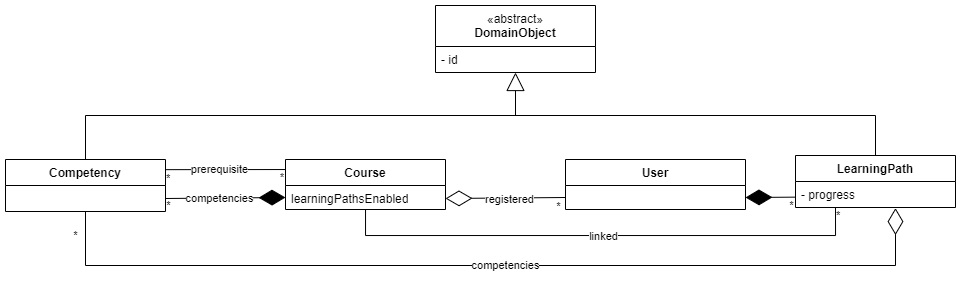
\includegraphics[width=\linewidth]{figures/LearningPathObjectModel.png}
	\caption{Class Diagram for the Composition of Learning Paths}
	\label{figure:LPOM}
\end{figure}

\section{Learning Path Graph}
\label{section:LearningPathGraph}

%------- chapter 7 -------

\chapter{Summary}

\textit{Note: This chapter includes the status of your thesis, a conclusion and an outlook about future work.}

\section{Status}

\textit{Note: Describe honestly the achieved goals (e.g. the well implemented and tested use cases) and the open goals here. if you only have achieved goals, you did something wrong in your analysis.}

\begin{itemize}
	\item [\Circle]
	\item [\LEFTcircle]
	\item [\CIRCLE]
\end{itemize}

\subsection{Realized Goals}

\textit{Note: Summarize the achieved goals by repeating the realized requirements or use cases stating how you realized them.}

\subsection{Open Goals}

\textit{Note: Summarize the open goals by repeating the open requirements or use cases and explaining why you were not able to achieve them. \textbf{Important:} It might be suspicious, if you do not have open goals. This usually indicates that you did not thoroughly analyze your problems.}

\section{Conclusion}

\textit{Note: Recap shortly which problem you solved in your thesis and discuss your \textbf{contributions} here.}

\section{Future Work}

\textit{Note: Tell us the next steps  (that you would do if you have more time). Be creative, visionary and open-minded here.}



\appendix

\chapter{e.g. Questionnaire}

\textit{Note: If you have large models, additional evaluation data like questionnaires or non summarized results, put them into the appendix.}


\clearpage

\listoffigures
\clearpage

\listoftables
\clearpage

\bibliography{thesis}
\bibliographystyle{alpha}

\end{document}
